\chapter{Interfaces, Surfactants and Colloids}\label{ch:b3:colloids}

Mayonnaise is oil dispersed as droplets a few micrometres across in a little
water and vinegar, held apart by the lecithin and proteins of egg yolk. Whisked
too fast at the start, or with the oil poured too quickly, it splits into an
oily layer and a watery one: the droplets merge, and the energy that kept them
apart is gone. Milk, fog, ink, paint, blood and the muddy water of a river are
the same kind of matter, particles or droplets far larger than molecules and
far smaller than anything the eye sees, so many that most of their molecules
are close to an interface. This chapter treats the energy of interfaces, the
molecules that lower it, the \omterm{def:b3:colloids:colloid}{colloids} that interfaces make possible, and what
keeps \omterm{def:b3:colloids:colloid}{colloids} dispersed or makes them coagulate.

\begin{recall}
The Year 1 volume called amphiphilic a molecule with a hydrophilic head and a
hydrophobic tail, and described London interactions and the relative
permittivity of solvents; the Grade 11 part of the first volume met \omterm{def:b3:colloids:micelle}{micelles}
in soap. The Year 2 volume defined the chemical potential, ionic strength and
activity. \Cref{ch:b3:surfaces-catalysis} treated \omterm{def:b3:surfaces-catalysis:adsorption}{adsorption} on solids,
\cref{ch:b3:electrode-kinetics} the \omterm{def:b3:electrode-kinetics:double-layer}{electrical double layer} and its \omterm{def:b3:electrode-kinetics:double-layer}{Debye
length}. From physics: Brownian motion, and the pressure inside a curved
surface.
\end{recall}

\begin{omfigure}
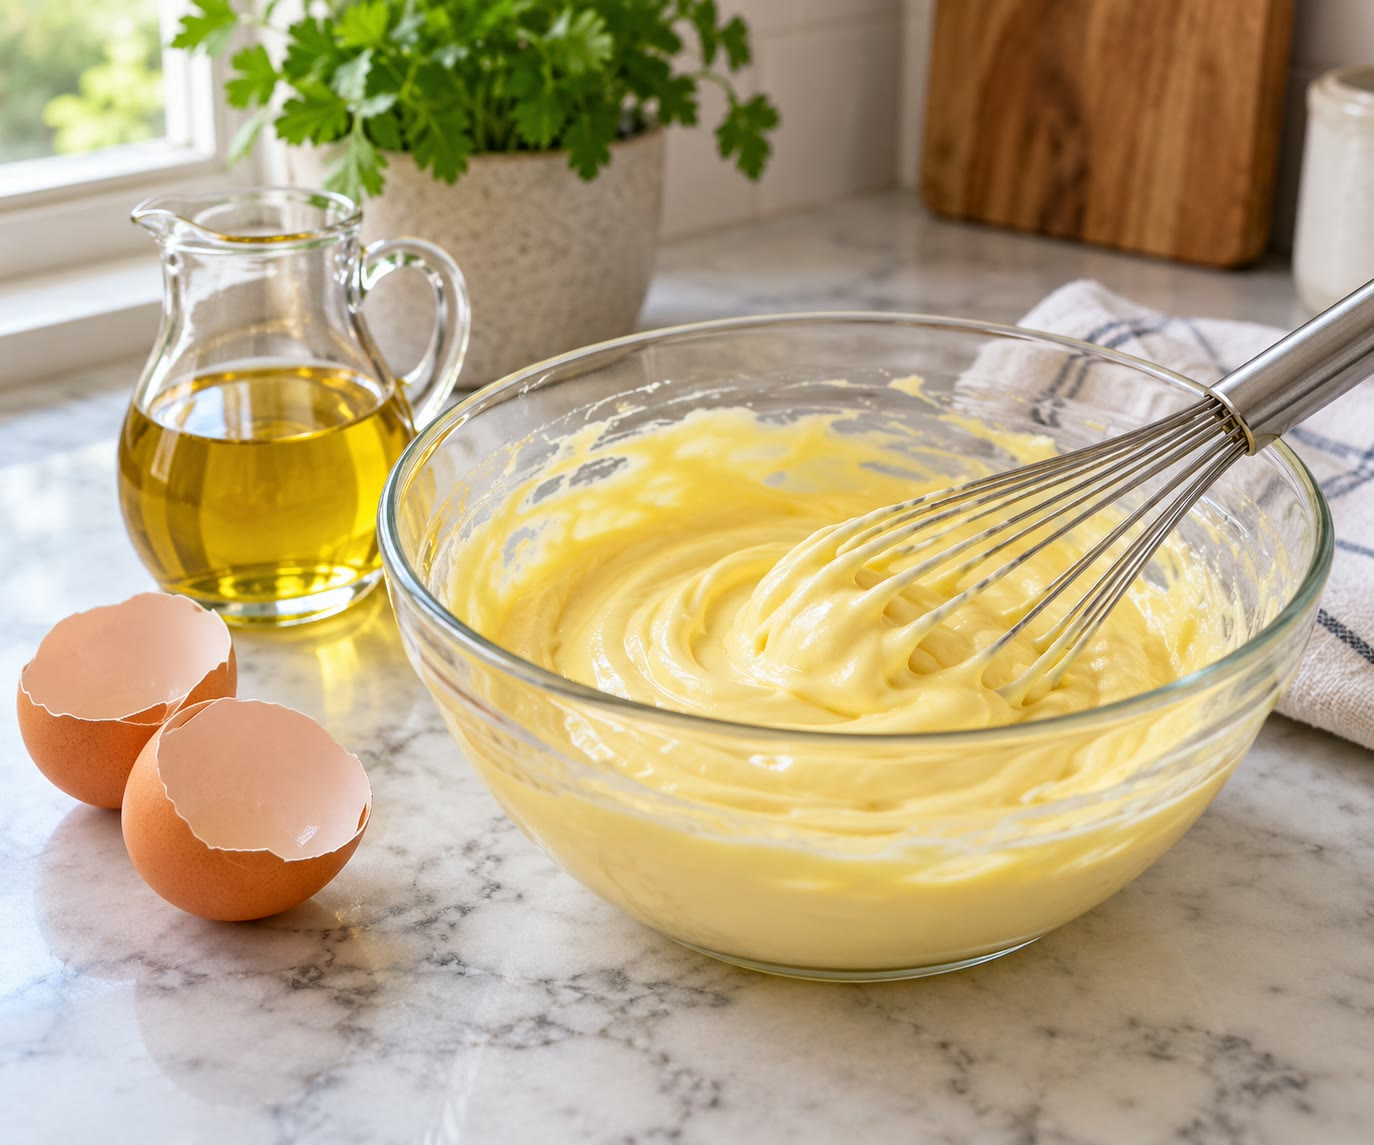
\includegraphics[width=0.6\linewidth]{images/book4/ai/b3-17-mayonnaise.jpg}

{\small Mayonnaise being whisked: an \omterm{def:b3:colloids:colloid}{emulsion} of oil droplets in water,
stabilised by the \omterm{def:b3:colloids:surfactant}{surfactants} of egg yolk.}
\end{omfigure}

\section{Interfaces and surface tension}

A molecule in the bulk of a liquid is attracted equally in all directions; at
the surface it loses part of its neighbours. Creating surface costs energy.

\begin{definition}[Surface tension]\label{def:b3:colloids:surface-tension}
The \emph{surface tension}\index{surface tension} $\gamma$ of a liquid is the Gibbs
energy needed to create a unit area of its surface at constant temperature,
pressure and composition: $\gamma = (\partial G/\partial A)_{T,p,n}$, in \unit{J.m^{-2}} $=$ \unit{N.m^{-1}}. For an
interface between two phases it is the interfacial tension.
\end{definition}

Water, held together by hydrogen bonds, has a high \omterm{def:b3:colloids:surface-tension}{surface tension}: \qty{72.0}{mN/m}
at \qty{25}{\celsius}. Alkanes have about 20, mercury about 480.

\begin{proposition}[Laplace pressure]\label{prop:b3:colloids:laplace}
The pressure inside a spherical drop or bubble of radius $r$ exceeds the
pressure outside by
\[
  \Delta p = \frac{2\gamma}{r} .
\]
\end{proposition}

\begin{proof}
Increase the radius by $\dd r$ at equilibrium: the work done by the pressure
difference, $\Delta p\,4\pi r^2\dd r$, equals the increase of surface Gibbs energy, $\gamma\,8\pi r\,\dd r$.
\end{proof}

\begin{definition}[Contact angle, wetting]\label{def:b3:colloids:wetting}
The \emph{contact angle}\index{contact angle} $\theta$ of a drop on a solid is the angle,
measured through the liquid, between the solid surface and the liquid surface
at the line where solid, liquid and vapour meet. A liquid \emph{wets}\index{wetting}
the solid when $\theta < 90^\circ$, and spreads completely when $\theta = 0$.
\end{definition}

\begin{theorem}[Young's equation]\label{thm:b3:colloids:young}
At equilibrium the three interfacial tensions and the \omterm{def:b3:colloids:wetting}{contact angle} satisfy
\[
  \gamma_{\mathrm{SV}} = \gamma_{\mathrm{SL}} + \gamma_{\mathrm{LV}}\cos\theta .
\]
This is \emph{Young's equation}\index{Young's equation}.
\end{theorem}

\begin{proof}
Move the contact line outwards by $\dd x$ (per unit length of line): solid--vapour
interface of area $\dd x$ is replaced by solid--liquid interface, and the
liquid--vapour interface grows by $\dd x\cos\theta$. The Gibbs energy changes by
$(\gamma_{\mathrm{SL}} - \gamma_{\mathrm{SV}} + \gamma_{\mathrm{LV}}\cos\theta)\dd x$, which is zero at equilibrium.
\end{proof}

\begin{omfigure}
\begin{tikzpicture}[font=\small, >=Stealth]
  \fill[black!12] (-3.6,-0.5) rectangle (3.6,0);
  \draw[thick] (-3.6,0) -- (3.6,0);
  \node[anchor=north] at (2.6,-0.05) {solid};
  \fill[omWater!60] (-2.0,0) arc[start angle=160, end angle=20, radius=2.13] -- cycle;
  \draw[thick, omDef] (-2.0,0) arc[start angle=160, end angle=20, radius=2.13];
  % circle centre 0.73 below the solid: a cap smaller than a hemisphere, contact angle 90 - 20 = 70 deg;
  % at the right contact point the liquid surface leaves at 110 deg (up and to the left)
  \draw[->, thick, omThm] (2.0,0) -- ++(110:1.3) node[anchor=south] {$\gamma_{\mathrm{LV}}$};
  \draw[->, thick] (2.0,0) -- (3.3,0) node[anchor=south] {$\gamma_{\mathrm{SV}}$};
  \draw[->, thick] (2.0,0) -- (0.7,0) node[anchor=north, yshift=-1pt] {$\gamma_{\mathrm{SL}}$};
  \draw (1.45,0) arc[start angle=180, end angle=110, radius=0.55];
  \node at (1.33,0.42) {$\theta$};
  \node at (0,0.6) {liquid};
  \node at (-2.8,1.4) {vapour};
\end{tikzpicture}

{\small A sessile drop and the three tensions pulling on its contact line: the
balance of their components along the solid gives \omterm{thm:b3:colloids:young}{Young's equation}; here $\theta
\approx 70^\circ$, a partially \omterm{def:b3:colloids:wetting}{wetting} liquid.}
\end{omfigure}

\begin{theorem}[Kelvin equation]\label{thm:b3:colloids:kelvin}
The vapour pressure of a spherical drop of radius $r$ exceeds that of the flat
liquid, $p^*$:
\[
  \ln\frac{p}{p^*} = \frac{2\gamma V_{\mathrm m}}{rRT},
\]
with $V_{\mathrm m}$ the molar volume of the liquid. This is the \emph{Kelvin
equation}\index{Kelvin equation}.
\end{theorem}

\begin{proof}
The liquid in the drop is under the extra pressure $2\gamma/r$, which raises its
chemical potential by $V_{\mathrm m}\,2\gamma/r$ (with $(\partial\mu/\partial p)_T = V_{\mathrm m}$, the liquid incompressible).
The vapour in equilibrium with it must have its chemical potential raised by
the same amount: $RT\ln(p/p^*) = 2\gamma V_{\mathrm m}/r$.
\end{proof}

For a water droplet of radius \qty{10}{nm} at \qty{25}{\celsius}, $2\gamma V_{\mathrm m}/rRT = 0.105$: its vapour
pressure is 11\,\% above that of flat water. Small droplets evaporate while
large ones grow, and clouds need nuclei to start; the same holds for the
solubility of small crystals.

\begin{definition}[Ostwald ripening]\label{def:b3:colloids:ripening}
\emph{Ostwald ripening}\index{Ostwald ripening} is the growth of the larger
particles or droplets of a dispersion at the expense of the smaller ones,
driven by the higher solubility or vapour pressure of small particles.
\end{definition}

\section{Surfactants and micelles}

\begin{definition}[Surfactant]\label{def:b3:colloids:surfactant}
A \emph{surfactant}\index{surfactant} (surface-active agent) is an amphiphilic
molecule that adsorbs at interfaces and lowers their tension. It is an
\emph{anionic surfactant}\index{anionic surfactant} if its head is an anion (sodium
dodecyl sulfate, soaps), a \emph{cationic surfactant}\index{cationic surfactant}
if a cation (quaternary ammonium salts), a \emph{non-ionic
surfactant}\index{non-ionic surfactant} if the head is a neutral polar group (a
chain of ethylene oxide units).
\end{definition}

\begin{definition}[Surface excess concentration]\label{def:b3:colloids:surface-excess}
The \emph{surface excess concentration}\index{surface excess concentration} $\Gamma$ of a
solute is the amount of solute at the interface per unit area, in excess of
what the same volume would hold if the bulk concentration held right up to
the interface.
\end{definition}

\begin{theorem}[Gibbs adsorption isotherm]\label{thm:b3:colloids:gibbs-adsorption}
For a dilute solution of a non-ionic solute of concentration $c$,
\[
  \Gamma = -\frac{1}{RT}\frac{\dd\gamma}{\dd\ln c};
\]
for a 1:1 ionic \omterm{def:b3:colloids:surfactant}{surfactant} without added salt, $RT$ is replaced by $2RT$. This is
the \emph{Gibbs adsorption isotherm}\index{Gibbs adsorption isotherm}.
\end{theorem}

\begin{proof}
For the interface, the analogue of the Gibbs--Duhem relation at constant $T$ and
$p$ is $\dd\gamma = -\sum_i\Gamma_i\,\dd\mu_i$ (the surface Gibbs energy $\gamma A$ plays the role of $G$,
admitted). Choosing the dividing surface so that the solvent has no excess,
$\dd\gamma = -\Gamma\,\dd\mu$, and in a dilute solution $\dd\mu = RT\,\dd\ln c$. For an ionic \omterm{def:b3:colloids:surfactant}{surfactant},
the cation and the anion are both adsorbed in equal excess and $\dd\mu$ becomes
$2RT\,\dd\ln c$.
\end{proof}

A \omterm{def:b3:colloids:surfactant}{surfactant} whose \omterm{def:b3:colloids:surface-tension}{surface tension} falls linearly with $\ln c$ has a constant
surface excess: the interface is saturated, and $1/(\Gamma N_A)$ is the area occupied by
one adsorbed molecule.

\begin{method}[Area per molecule from a $\gamma$--$\ln c$ slope]\label{met:b3:colloids:surface-excess}
\begin{enumerate}
  \item Measure $\gamma$ against $c$ below the CMC; plot $\gamma$ against $\ln c$.
  \item Take the slope of the linear part just below the CMC; $\Gamma = -\text{slope}/(nRT)$, $n
        = 1$ for a \omterm{def:b3:colloids:surfactant}{non-ionic surfactant}, 2 for a 1:1 ionic one without salt.
  \item Area per molecule $= 1/(\Gamma N_A)$; typical values are 0.3 to \qty{0.6}{nm^2}.
\end{enumerate}
\end{method}

\begin{definition}[Micelle, critical micelle concentration, aggregation number]\label{def:b3:colloids:micelle}
A \emph{micelle}\index{micelle} is an aggregate of \omterm{def:b3:colloids:surfactant}{surfactant} molecules in solution
whose hydrophobic tails form a liquid-like core shielded from water by the
heads. The \emph{critical micelle concentration}\index{critical micelle concentration}
(CMC) is the concentration above which micelles form; their
mean number of molecules is the \emph{aggregation number}\index{aggregation number}.
\end{definition}

\begin{proposition}[Breaks at the CMC]\label{prop:b3:colloids:cmc-break}
Above the CMC, the concentration of free \omterm{def:b3:colloids:surfactant}{surfactant}, and with it the \omterm{def:b3:colloids:surface-tension}{surface
tension} and the osmotic pressure, stay almost constant; properties that depend
on the free molecules change slope at the CMC.
\end{proposition}

\begin{proof}[Partial proof]
Treat the \omterm{def:b3:colloids:micelle}{micelles} as a separate phase: added \omterm{def:b3:colloids:surfactant}{surfactant} goes into \omterm{def:b3:colloids:micelle}{micelles} once
the chemical potential of the free molecules reaches that of a molecule in a
\omterm{def:b3:colloids:micelle}{micelle}, and this chemical potential, hence the free concentration, then stays
fixed. The \omterm{def:b3:colloids:surface-tension}{surface tension}, set by the free molecules through the Gibbs
isotherm, stops falling; the conductivity keeps rising, but more slowly, since
\omterm{def:b3:colloids:micelle}{micelles} carry less charge per \omterm{def:b3:colloids:surfactant}{surfactant} than free ions (part of their
counterions are bound). The model is a limit, since \omterm{def:b3:colloids:micelle}{micelles} of finite size
form over a narrow range of concentration (admitted).
\end{proof}

\begin{method}[The CMC from a break]\label{met:b3:colloids:cmc}
\begin{enumerate}
  \item Measure the \omterm{def:b3:colloids:surface-tension}{surface tension} (or, for an ionic \omterm{def:b3:colloids:surfactant}{surfactant}, the
        conductivity) over a range of concentrations spanning the expected
        CMC.
  \item Fit straight lines to the two branches ($\gamma$ against $\log c$, or $\kappa$ against $c$).
  \item Their intersection is the CMC.
\end{enumerate}
\end{method}

\begin{omfigure}
\begin{tikzpicture}
\begin{axis}[name=gm, width=0.47\linewidth, height=5.2cm, xmin=-5, xmax=-1.5, ymin=30, ymax=76,
  axis lines=left, xlabel={$\log(c/\unit{mol.L^{-1}})$}, ylabel={$\gamma$ / \unit{mN.m^{-1}}},
  tick label style={font=\small}, label style={font=\small}]
\addplot[omDef, very thick] table[x=logc, y=gamma_mN] {figdata/out/bachelor-3-surfactant-cmc-gamma.dat};
\draw[black!40, dashed] (axis cs:-2.086,30) -- (axis cs:-2.086,70);
\node[font=\scriptsize, anchor=south west] at (axis cs:-2.05,45) {CMC};
\end{axis}
\begin{axis}[at={(gm.east)}, anchor=west, xshift=1.4cm, width=0.47\linewidth, height=5.2cm,
  xmin=0, xmax=20, ymin=0, ymax=1.0, axis lines=left, xlabel={$c$ / mM},
  ylabel={$\kappa$ / \unit{mS.cm^{-1}}}, tick label style={font=\small}, label style={font=\small}]
\addplot[omThm, very thick] table[x=c_mM, y=kappa] {figdata/out/bachelor-3-surfactant-cmc-kappa.dat};
\draw[black!40, dashed] (axis cs:8.2,0) -- (axis cs:8.2,0.9);
\node[font=\scriptsize, anchor=south west] at (axis cs:8.4,0.15) {CMC};
\end{axis}
\end{tikzpicture}

{\small A model ionic \omterm{def:b3:colloids:surfactant}{surfactant} with the CMC of sodium dodecyl sulfate,
\qty{8.2}{mM} at \qty{25}{\celsius}. Left: the \omterm{def:b3:colloids:surface-tension}{surface tension} falls with $\log c$, linearly just below
the CMC (a saturated interface, area about \qty{0.6}{nm^2} per molecule), then stays
constant. Right: the conductivity rises less steeply above the CMC.}
\end{omfigure}

\begin{definition}[Packing parameter]\label{def:b3:colloids:packing}
The \emph{packing parameter}\index{packing parameter} of a \omterm{def:b3:colloids:surfactant}{surfactant} is $P =
v/(a_0l)$, where $v$ is the volume of its hydrophobic tail, $l$ the length of the
extended tail and $a_0$ the optimal area per head group at the aggregate
surface.
\end{definition}

\begin{proposition}[Shape of aggregates]\label{prop:b3:colloids:packing}
Spherical \omterm{def:b3:colloids:micelle}{micelles} need $P \le \frac13$, cylindrical \omterm{def:b3:colloids:micelle}{micelles} $\frac13 < P \le \frac12$, flat bilayers
(vesicles, membranes) $\frac12 < P \le 1$; $P > 1$ gives reversed structures.
\end{proposition}

\begin{proof}
In a sphere of radius $R \le l$ made of $N$ molecules, $Nv = \frac43\pi R^3$ and $Na_0 = 4\pi R^2$, so
$v/a_0 = R/3 \le l/3$: $P \le \frac13$. For a cylinder of radius $R$ and length $L$, $Nv = \pi R^2L$ and
$Na_0 = 2\pi RL$: $v/a_0 = R/2 \le l/2$. For a bilayer of thickness $2l$ and area $A$, $Nv = 2lA$ and
$Na_0 = 2A$: $v/a_0 = l$.
\end{proof}

\begin{omfigure}
\begin{tikzpicture}[font=\scriptsize]
  % a sphere-forming cone
  \draw[omDef, thick, fill=omDef!15] (0,0) -- (-0.45,1.2) arc[start angle=180, end angle=0, radius=0.45] -- cycle;
  \node at (0,-0.3) {$P < \frac13$: cone};
  % micelle
  \begin{scope}[xshift=2.2cm, yshift=0.6cm]
    \foreach \a in {0,30,...,330}{\draw[black!60] (\a:0.2) -- (\a:0.62); \fill[omDef] (\a:0.7) circle (0.09);}
    \node at (0,-1.05) {spherical micelle};
  \end{scope}
  % truncated cone
  \begin{scope}[xshift=4.7cm]
    \draw[omDef, thick, fill=omDef!15] (-0.18,0) -- (-0.4,1.2) -- (0.4,1.2) -- (0.18,0) -- cycle;
    \node at (0,-0.3) {$\frac13 < P < \frac12$};
  \end{scope}
  \begin{scope}[xshift=6.9cm, yshift=0.6cm]
    \fill[omDef!10] (-0.9,-0.55) rectangle (0.9,0.55);
    \foreach \x in {-0.8,-0.5,...,0.8}{\fill[omDef] (\x,0.62) circle (0.08); \fill[omDef] (\x,-0.62) circle (0.08);}
    \node at (0,-1.05) {cylinder (side view)};
  \end{scope}
  % cylinder shape
  \begin{scope}[xshift=9.4cm]
    \draw[omDef, thick, fill=omDef!15] (-0.3,0) rectangle (0.3,1.2);
    \node at (0,-0.3) {$P \approx 1$: cylinder};
  \end{scope}
  \begin{scope}[xshift=11.4cm, yshift=0.6cm]
    \foreach \x in {-0.8,-0.6,...,0.8}{
      \draw[black!60] (\x,0.5) -- (\x,0.05) (\x,-0.5) -- (\x,-0.05);
      \fill[omDef] (\x,0.58) circle (0.08); \fill[omDef] (\x,-0.58) circle (0.08);}
    \node at (0,-1.05) {bilayer};
  \end{scope}
\end{tikzpicture}

{\small Molecular shape and aggregate shape. A \omterm{def:b3:colloids:surfactant}{surfactant} with a large head and
a single tail (a cone) packs into spherical \omterm{def:b3:colloids:micelle}{micelles}; a smaller head into
cylinders; a molecule as wide at the tail as at the head, such as a lipid with
two chains, into flat bilayers, the walls of vesicles and cell membranes.}
\end{omfigure}

Detergency combines these effects: the \omterm{def:b3:colloids:surfactant}{surfactant} lowers the interfacial
tension between water and an oily soil until the soil rolls up into drops,
which \omterm{def:b3:colloids:micelle}{micelles} then solubilise in their cores.

\section{Colloids}

\begin{definition}[Colloid]\label{def:b3:colloids:colloid}
A \emph{colloid}\index{colloid} is a dispersion of particles, droplets or bubbles,
roughly \qty{1}{nm} to \qty{1}{\micro m} across (the \emph{dispersed phase}\index{dispersed phase}),
in a continuous \emph{dispersion medium}\index{dispersion medium}. A
\emph{sol}\index{sol} is a dispersion of solid particles in a liquid, an
\emph{emulsion}\index{emulsion} of liquid droplets in another liquid, a
\emph{foam}\index{foam} of gas bubbles in a liquid or a solid, a \emph{gel}\index{gel}
a network of particles or polymers that spans the whole liquid and makes it
solid-like, an \emph{aerosol}\index{aerosol} of droplets or particles in a gas.
\end{definition}

Colloidal particles are small enough to stay suspended by Brownian motion (the
random kicks of solvent molecules, from physics) and large enough to scatter
light.

\begin{definition}[Tyndall effect]\label{def:b3:colloids:tyndall}
The \emph{Tyndall effect}\index{Tyndall effect} is the scattering of light by the
particles of a \omterm{def:b3:colloids:colloid}{colloid}, which makes a beam visible from the side when it
crosses the \omterm{def:b3:colloids:colloid}{colloid}, while a true solution remains invisible.
\end{definition}

\begin{omfigure}
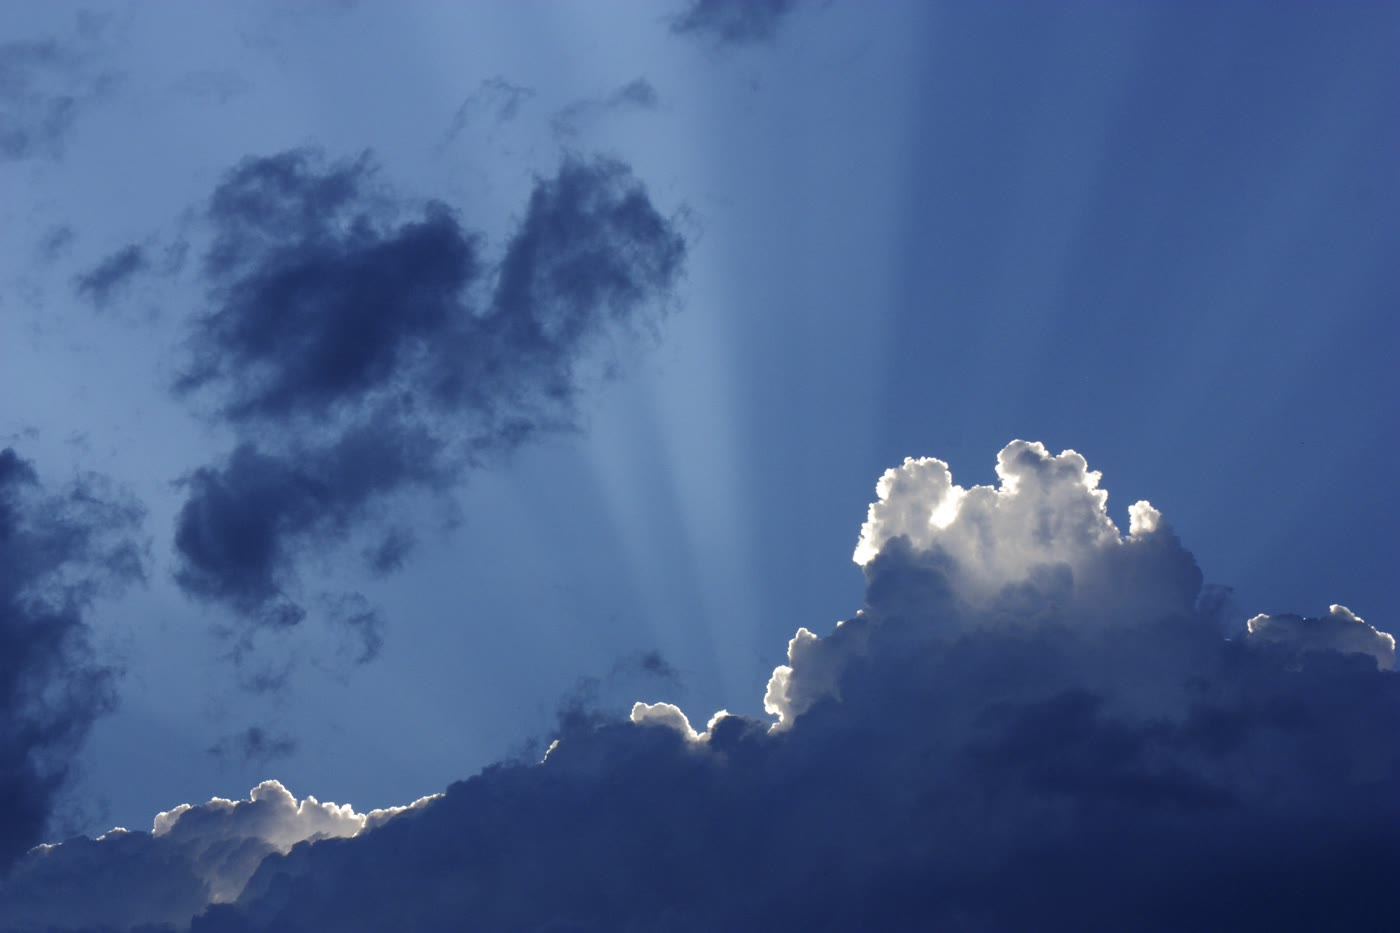
\includegraphics[width=0.55\linewidth]{images/book4/tyndall-sky.jpg}

{\small Sunbeams through a gap in the clouds: they are visible because the
\omterm{def:b3:colloids:colloid}{aerosol} of the air, droplets and dust, scatters part of the light sideways, the
\omterm{def:b3:colloids:tyndall}{Tyndall effect} on the scale of the sky.}
\end{omfigure}

\section{Colloidal stability}

Two colloidal particles always attract each other at short range by van der
Waals forces. In water, most particles also carry a charge (ionised surface
groups, adsorbed ions), surrounded by a \omterm{def:b3:electrode-kinetics:double-layer}{diffuse layer} of counterions, the double
layer of \cref{ch:b3:electrode-kinetics}. When two particles approach, their
\omterm{def:b3:electrode-kinetics:double-layer}{diffuse layers} overlap and repel.

\begin{definition}[Zeta potential]\label{def:b3:colloids:zeta}
The \emph{zeta potential}\index{zeta potential} $\zeta$ of a particle is the electric
potential at its slipping plane, the boundary within the double layer between
the liquid that moves with the particle and the liquid that does not; it is
measured from the velocity of the particles in an electric field
(electrophoresis).
\end{definition}

\begin{omfigure}
\begin{tikzpicture}[font=\scriptsize]
  \fill[black!20] (0,0) circle (1.2);
  \foreach \a in {0,30,...,330}{\node at (\a:1.05) {$-$};}
  \draw[omDef, dashed] (0,0) circle (1.55);
  \foreach \a in {15,45,...,345}{\draw[omDef, fill=omDef!15] (\a:1.38) circle (0.11); \node at (\a:1.38) {\tiny$+$};}
  \draw[omThm, thick, densely dotted] (0,0) circle (1.85);
  \foreach \a/\r/\s in {10/2.2/+, 50/2.5/+, 95/2.3/-, 130/2.7/+, 175/2.2/+, 215/2.6/-, 250/2.3/+, 290/2.8/+, 345/2.6/+}{
    \draw[black!60, fill=white] (\a:\r) circle (0.11); \node at (\a:\r) {\tiny$\s$};}
  \draw[->, black!60] (2.6,1.6) node[anchor=west] {Stern layer} -- (40:1.6);
  \draw[->, omThm] (2.6,-1.4) node[anchor=west] {slipping plane: $\zeta$} -- (-30:1.87);
  \node at (0,0) {particle};
  \node[anchor=west] at (2.9,0.2) {diffuse layer};
\end{tikzpicture}

{\small A negatively charged particle with its double layer: a compact Stern
layer of counterions, the slipping plane just beyond it, where the \omterm{def:b3:colloids:zeta}{zeta
potential} is defined, and the \omterm{def:b3:electrode-kinetics:double-layer}{diffuse layer}, in which counterions outnumber
co-ions over a few \omterm{def:b3:electrode-kinetics:double-layer}{Debye lengths}.}
\end{omfigure}

\begin{theorem}[DLVO theory]\label{thm:b3:colloids:dlvo}
For two spheres of radius $a$ separated by a gap $h \ll a$, with diffuse-layer potential
$\psi$ and Hamaker constant $A$, the interaction energy is, for low potentials,
\[
  V(h) = 2\pi\varepsilon_r\varepsilon_0a\psi^2\ln\bigl(1 + \eu^{-\kappa h}\bigr) - \frac{Aa}{12h} .
\]
The first term, the double-layer repulsion, decays over the \omterm{def:b3:electrode-kinetics:double-layer}{Debye length} $\kappa^{-1}$;
the second, the van der Waals attraction, does not depend on the salt. Their sum
has an energy barrier at a few \omterm{def:b3:electrode-kinetics:double-layer}{Debye lengths} when the salt concentration is
low, and none above a critical concentration.
\end{theorem}

\begin{proof}[Partial proof]
Both forms are admitted (the repulsion from the overlap of two Gouy--Chapman
layers in the Derjaguin approximation, the attraction from summing London
interactions over the two bodies). Raising the ionic strength raises $\kappa$
(\cref{prop:b3:electrode-kinetics:debye-length}): the repulsion then dies out at
smaller $h$, where the attraction, which grows as $1/h$, is stronger; the maximum
of $V$ decreases and finally vanishes.
\end{proof}

\begin{omfigure}
\begin{tikzpicture}
\begin{axis}[width=0.72\linewidth, height=5.6cm, xmin=0, xmax=30, ymin=-40, ymax=45,
  axis lines=left, xlabel={gap $h$ / nm}, ylabel={$V/kT$},
  tick label style={font=\small}, label style={font=\small},
  legend style={font=\scriptsize, draw=none, at={(0.98,0.98)}, anchor=north east}, legend cell align=left]
\addplot[omDef, thick] table[x=h_nm, y=I1] {figdata/out/bachelor-3-dlvo.dat};
\addplot[black!60, thick] table[x=h_nm, y=I10] {figdata/out/bachelor-3-dlvo.dat};
\addplot[omThm, thick] table[x=h_nm, y=I50] {figdata/out/bachelor-3-dlvo.dat};
\addplot[black, thick, dashed] table[x=h_nm, y=I200] {figdata/out/bachelor-3-dlvo.dat};
\draw[black!30] (axis cs:0,0) -- (axis cs:30,0);
\legend{\qty{1}{mM}, \qty{10}{mM}, \qty{50}{mM}, \qty{200}{mM}}
\end{axis}
\end{tikzpicture}

{\small DLVO interaction of two particles of radius \qty{100}{nm} (model: diffuse-layer
potential \qty{-30}{mV}, Hamaker constant \qty{2e-20}{J}) in water with a 1:1 salt. At \qty{1}{mM}
a barrier of about $40\,kT$ keeps the particles apart; at \qty{10}{mM} it is halved;
near \qty{50}{mM} it disappears and every collision is sticky.}
\end{omfigure}

\begin{definition}[Coagulation and stabilisation]\label{def:b3:colloids:stability}
\emph{Coagulation}\index{coagulation} is the aggregation of colloidal particles
caused by the loss of their electrostatic repulsion; \emph{flocculation}\index{flocculation}
is aggregation into loose flocs, often bridged by adsorbed polymers. The
\emph{critical coagulation concentration}\index{critical coagulation concentration}
(CCC) of an electrolyte is the concentration above which a
\omterm{def:b3:colloids:colloid}{colloid} coagulates rapidly. \emph{Steric stabilisation}\index{steric stabilisation}
keeps particles apart with adsorbed or grafted polymer chains,
whose overlap would cost entropy.
\end{definition}

\begin{proposition}[Schulze--Hardy rule]\label{prop:b3:colloids:schulze-hardy}
For a highly charged \omterm{def:b3:colloids:colloid}{colloid}, the \omterm{def:b3:colloids:stability}{critical coagulation concentration} of an
electrolyte varies as the inverse sixth power of the charge $z$ of its
counterions: $\text{CCC} \propto z^{-6}$, in the ratios $1 : \frac{1}{64} : \frac{1}{729}$ for $z = 1, 2, 3$.
\end{proposition}

\begin{proof}[Partial proof]
Treat two flat plates. At high surface potential the double-layer repulsion per
unit area tends to $V_R = (64nkT/\kappa)\eu^{-\kappa h}$, where $n$ is the number density of the $z{:}z$
electrolyte, independent of the potential (admitted); the attraction is $V_A =
-A/(12\pi h^2)$. At the CCC the barrier just vanishes: $V = 0$ and $\dd V/\dd h = 0$ at the same
gap. Since $\dd V_R/\dd h = -\kappa V_R$ and $\dd V_A/\dd h = -2V_A/h$, the two conditions give
$\kappa V_R = 2V_R/h$, so $\kappa h = 2$, and then $64nkT\eu^{-2}/\kappa = A\kappa^2/(48\pi)$, i.e. $n \propto \kappa^3$. With
$\kappa^2 = 2nz^2e^2/(\varepsilon kT)$, $\kappa^3 \propto (nz^2)^{3/2}$ and $n \propto n^{3/2}z^3$: hence $n \propto z^{-6}$.
\end{proof}

\begin{omfigure}
\begin{tikzpicture}[font=\small, >=Stealth]
  \foreach \x/\lab/\v in {0/\ce{Na+}/1, 2.6/\ce{Ca^{2+}}/{1/64}, 5.2/\ce{Al^{3+}}/{1/729}}{
    \node at (\x,0) {\lab};
    \node[font=\scriptsize] at (\x,-0.45) {CCC $\times\,\v$};}
  \draw[->, thick, omDef] (-0.8,-0.95) -- (6.0,-0.95) node[midway, below, font=\scriptsize] {smaller dose to coagulate a negative colloid};
\end{tikzpicture}

{\small The Schulze--Hardy rule for a negatively charged \omterm{def:b3:colloids:colloid}{colloid}: the \omterm{def:b3:colloids:stability}{critical
coagulation concentration} falls as the sixth power of the counterion charge.}
\end{omfigure}

The rule explains why aluminium salts are so effective at clearing water, and
why rivers drop their load of clay where they meet the salt water of the sea.

\begin{method}[Choosing a coagulant dose]\label{met:b3:colloids:coagulant-dose}
\begin{enumerate}
  \item Measure the CCC of a reference electrolyte for the suspension (jar tests
        with increasing doses, watching the settling).
  \item Scale it to the counterion of the coagulant with the Schulze--Hardy rule.
  \item Convert to a mass of salt per cubic metre with its formula; add enough
        for the hydrolysis and the alkalinity it consumes.
  \item Avoid overdosing: highly charged counterions can reverse the sign of
        the particles' charge and restabilise them.
\end{enumerate}
\end{method}

\section{Colloids at work}

\begin{definition}[Hydrophilic--lipophilic balance]\label{def:b3:colloids:hlb}
The \emph{hydrophilic--lipophilic balance}\index{hydrophilic--lipophilic balance}
(HLB) of a \omterm{def:b3:colloids:surfactant}{non-ionic surfactant} is, in Griffin's scale, $20$ times the mass
fraction of its hydrophilic part: low values (3 to 6) suit water-in-oil
\omterm{def:b3:colloids:colloid}{emulsions}, high values (8 to 18) oil-in-water \omterm{def:b3:colloids:colloid}{emulsions} and detergents.
\end{definition}

\omterm{def:b3:colloids:colloid}{Emulsions} are thermodynamically unstable, since every droplet carries
interfacial energy; emulsifiers make them kinetically stable by lowering that
energy and by adding a repulsive layer, charged or steric, around each droplet.
Mayonnaise is an oil-in-water \omterm{def:b3:colloids:colloid}{emulsion} with so much oil (about four fifths of
the volume) that the droplets are squeezed against one another, which makes it
a soft solid. \omterm{def:b3:colloids:colloid}{Foams} are stabilised by \omterm{def:b3:colloids:surfactant}{surfactants} that slow the draining of the
liquid films between bubbles; antifoams, often silicone oils, spread on those
films and break them. In drinking-water plants, aluminium or iron(III) salts
coagulate the clay and organic \omterm{def:b3:colloids:colloid}{colloids} that make river water turbid; the
hydroxide they form sweeps the flocs down as it settles. Metal nanoparticles
are kept dispersed by adsorbed citrate ions (electrostatic) or by thiol-bound
polymer chains (steric).

\begin{inthelab}[The du Noüy ring]
A platinum ring, flamed to clean it, hangs from a balance and is immersed
horizontally in the liquid, then slowly raised. The force needed to pull it
through the surface passes a maximum; divided by twice the circumference of
the ring and corrected for the shape of the lifted meniscus, it gives the
\omterm{def:b3:colloids:surface-tension}{surface tension}. The measurement of a \omterm{def:b3:colloids:surfactant}{surfactant} series starts from the most
dilute solution, rinsing the ring between samples.
\end{inthelab}

\begin{safety}{\ghs[0.8cm]{GHS02}\ghs[0.8cm]{GHS05}\ghs[0.8cm]{GHS07}}
% ledger: ghs4:SDS, ghs4:Al2SO43
Sodium dodecyl sulfate powder: flammable solid, harmful if swallowed, causes
serious eye damage, irritates the respiratory tract; weighed without raising
dust, with eye protection. Aluminium sulfate (\ghs[0.6cm]{GHS05}): causes serious eye
damage.
\end{safety}

\begin{history}[Tyndall and the ultramicroscope]
John Tyndall showed in 1869 that a beam of light becomes visible in air laden
with fine particles and invisible in air freed of them, and that the scattered
light is bluish and polarised. Richard Zsigmondy, studying the red colour of
gold \omterm{def:b3:colloids:colloid}{sols}, built with Henry Siedentopf in 1903 the ultramicroscope, which lights
the \omterm{def:b3:colloids:colloid}{colloid} from the side and shows each particle as a point of scattered light
on a dark background, too small to be resolved but countable. He received the
1925 Nobel Prize in Chemistry for his work on \omterm{def:b3:colloids:colloid}{colloids}.
\end{history}

\section{Exercises}

\begin{exercise}[$\star$]\label{exo:b3:colloids:1}
% ledger: st:H2O.25C
Compute the pressure inside an air bubble of diameter \qty{1.0}{\micro m} in water at
\qty{25}{\celsius} (outside: \qty{1.0}{bar}).
\end{exercise}

\begin{exercise}[$\star$]\label{exo:b3:colloids:2}
% ledger: st:H2O.25C
Compute the vapour pressure of a water droplet of radius \qty{10}{nm} relative to
flat water at \qty{25}{\celsius} ($V_{\mathrm m} = \qty{18.07}{cm^3/mol}$).
\end{exercise}

\begin{exercise}[$\star$]\label{exo:b3:colloids:3}
A liquid with $\gamma_{\mathrm{LV}} = \qty{72}{mN/m}$ on a solid with $\gamma_{\mathrm{SV}} = \qty{40}{mN/m}$ and $\gamma_{\mathrm{SL}} =
\qty{20}{mN/m}$ (data of the exercise): compute the \omterm{def:b3:colloids:wetting}{contact angle}. Does it wet?
\end{exercise}

\begin{exercise}[$\star$]\label{exo:b3:colloids:4}
% ledger: eps:H2O.25C
Compute the \omterm{def:b3:electrode-kinetics:double-layer}{Debye length} in water at \qty{25}{\celsius} for \qty{0.010}{mol/L} of NaCl and of
\ce{MgSO4}.
\end{exercise}

\begin{exercise}[$\star\star$]\label{exo:b3:colloids:5}
Just below its CMC, the \omterm{def:b3:colloids:surface-tension}{surface tension} of an ionic \omterm{def:b3:colloids:surfactant}{surfactant} (1:1, no salt)
falls by \qty{12.6}{mN/m} per unit of $\ln c$ at \qty{25}{\celsius}. Compute the surface excess and
the area per molecule.
\end{exercise}

\begin{exercise}[$\star\star$]\label{exo:b3:colloids:6}
\omterm{def:b3:colloids:surface-tension}{Surface tensions} of a \omterm{def:b3:colloids:surfactant}{non-ionic surfactant}: 52.0, 45.5, 39.1, 33.4, 33.3 and
\qty{33.4}{mN/m} at $\log c = -5.0$, $-4.5$, $-4.0$, $-3.5$, $-3.0$ and $-2.5$ (data of the exercise).
Estimate the CMC.
\end{exercise}

\begin{exercise}[$\star\star$]\label{exo:b3:colloids:7}
For sodium dodecyl sulfate, take $v = \qty{0.350}{nm^3}$, $l = \qty{1.67}{nm}$ and $a_0 = \qty{0.60}{nm^2}$; for a
lipid with two such chains, $2v$, the same $l$ and $a_0 = \qty{0.65}{nm^2}$ (data of the
exercise). Predict the shape of their aggregates.
\end{exercise}

\begin{exercise}[$\star\star$]\label{exo:b3:colloids:8}
A negatively charged \omterm{def:b3:colloids:colloid}{sol} coagulates at \qty{60}{mM} NaCl. Predict the CCC with \ce{CaCl2}
and with \ce{AlCl3}. What would \ce{Na3PO4} do?
\end{exercise}

\begin{exercise}[$\star\star$]\label{exo:b3:colloids:9}
% ledger: cmc:C12E6
Compute Griffin's HLB of hexaethylene glycol monododecyl ether,
\ce{C12H25(OCH2CH2)6OH}, whose hydrophilic part is $\ce{(OCH2CH2)6OH}$. Is it suited to an
oil-in-water \omterm{def:b3:colloids:colloid}{emulsion}?
\end{exercise}

\begin{exercise}[$\star\star\star$]\label{exo:b3:colloids:10}
A dispersion contains droplets of radius 50 and \qty{500}{nm}. Using the \omterm{thm:b3:colloids:kelvin}{Kelvin
equation} applied to solubility, explain which grow and which shrink, and why
\omterm{def:b3:colloids:colloid}{emulsions} coarsen with time even without coalescence.
\end{exercise}

\begin{exercise}[$\star\star\star$]\label{exo:b3:colloids:11}
Show from the Laplace pressure that the liquid rises to the height $h = 2\gamma\cos\theta/(\rho gr)$ in a
capillary of radius $r$, and compute it for water ($\theta = 0$, \qty{0.10}{mm} radius).
\end{exercise}

\begin{exercise}[$\star\star\star$]\label{exo:b3:colloids:12}
Using the DLVO figure, explain why adding \qty{100}{mM} NaCl to a \omterm{def:b3:colloids:colloid}{sol} stable at \qty{1}{mM}
makes it coagulate, while adding a non-adsorbing polymer does not change the
barrier but a polymer grafted to the particles can keep them apart at any salt
concentration.
\end{exercise}

% keep the heading with its problem box, which fills a page by itself
\clearpage
\enlargethispage{3\baselineskip}
\section{Problem: Clearing Muddy Water with Alum}

\begin{problem}[{Weekend problem --- clearing muddy water with alum: the
double layer of clay particles, the DLVO barrier, the Schulze--Hardy rule, and
the dose of aluminium sulfate}]
\label{pb:b3:colloids:1}
% ledger: eps:H2O.25C, visc:H2O.25C
A water-treatment plant receives soft, turbid water: clay particles of radius
\qty{100}{nm} and density \qty{2650}{kg/m^3}, with a diffuse-layer potential of \qty{-30}{mV}, in
water containing \qty{1.0}{mM} of \ce{NaHCO3}. Jar tests show that the particles coagulate
rapidly above \qty{50}{mM} of NaCl (data of the problem). The plant treats \qty{1000}{m^3} per
hour with aluminium sulfate, $\ce{Al2(SO4)3}$ ($M = \qty{342.3}{g/mol}$).

\medskip\noindent\textbf{Part I --- A stable \omterm{def:b3:colloids:colloid}{colloid}.}
\begin{enumerate}
  \item Why do clay particles in water carry a negative charge?
  \item Compute the ionic strength of the water.
  \item Compute its \omterm{def:b3:electrode-kinetics:double-layer}{Debye length}.
  \item Compare it with the particle radius. Which approximation of the DLVO
        formula does this justify?
  \item Compute the settling velocity of a particle by Stokes' law, $v =
        2\Delta\rho\,gr^2/9\eta$ ($\eta = \qty{0.89}{mPa.s}$), in millimetres per day.
  \item Why do the particles not stick together when they collide?
\end{enumerate}

\medskip\noindent\textbf{Part II --- The DLVO barrier.}
\begin{enumerate}[resume]
  \item Write the DLVO energy of two particles.
  \item Read on the figure the barrier at \qty{1}{mM}, in units of $kT$.
  \item How often would two colliding particles cross such a barrier?
  \item What happens to the barrier near \qty{50}{mM}?
  \item Explain why adding salt lowers the barrier.
\end{enumerate}

\medskip\noindent\textbf{Part III --- Schulze--Hardy.}
\begin{enumerate}[resume]
  \item State the rule.
  \item Predict the CCC of \ce{Ca^{2+}}.
  \item Predict the CCC of \ce{Al^{3+}}.
  \item Why do only the cations of the coagulant matter for this \omterm{def:b3:colloids:colloid}{colloid}?
  \item Why is the sulfate of alum nearly irrelevant to the \omterm{def:b3:colloids:stability}{coagulation}?
\end{enumerate}

\medskip\noindent\textbf{Part IV --- The dose.}
\begin{enumerate}[resume]
  \item Compute the amount of \ce{Al^{3+}} needed per cubic metre.
  \item Deduce the amount of $\ce{Al2(SO4)3}$ per cubic metre.
  \item Deduce its mass per cubic metre.
  \item Deduce the mass used per hour by the plant.
  \item In water, \ce{Al^{3+}} hydrolyses and reacts with the hydrogencarbonate. Write the
        balanced equation forming \ce{Al(OH)3}.
  \item What fraction of the hydrogencarbonate does the dose consume? Does the
        pH change much?
  \item Why can an overdose make the water turbid again?
  \item State the result: the minimum mass of aluminium sulfate per cubic metre.
\end{enumerate}
\end{problem}
